\documentclass{article}
\usepackage[utf8]{inputenc}
\usepackage[margin=1in]{geometry}

\usepackage{graphicx}
\usepackage{wrapfig}


\title{Splay Trees}
\author{Kevin Geng and Lawrence Wang}
\date{17 February 2017}

\begin{document}

\maketitle

\section{Balancing BSTs}

Binary search trees allow us to store a sequence of elements in sorted order, and search for and update them in logarithmic time. One problem with BSTs is the difficulty of keeping a tree balanced: operations on an unbalanced tree could degenerate to $O(N)$. To solve this, there are several different methods of balancing BSTs, to ensure that their maximum height never exceeds a logarithmic factor, bounding all of our operations to $O(\log N)$.

One reason we might want to build our own balanced BST is to implement operations that the standard library implementation doesn't provide. For example, one way to solve the intersecting lines problem is with a line sweep in $O(N \log N)$ by augmenting a binary search tree with subtree sizes. However, \verb|std::set| doesn't provide us with this information, so we need to implement our own tree.

\section{Splay trees}

A splay tree balances itself by reorganizing it after every operation (including insertion, query, etc.). Specifically, after inserting some element $x$, we will rotate $x$ to the root of the tree using tree rotations. This operation is called \textit{splaying}, and it turns out that this keeps the tree relatively balanced most of the time. We can use the fact that we splay after every operation to implement various operations easily.

Another property of splay trees is that recently accessed elements are near the top of the tree, for obvious reasons. This gives an additional performance benefit if some items are accessed more frequently than others, though splay trees are still useful even without this property.

\section{Splay operation}

A splay operation moves some node $x$ to the root of the tree. To do this, we break it down into a series of \textit{splay steps}, each of which moves a node up one level. The step we need to perform depends on whether $x$ is a left or right child of its parent $p$, and whether $p$ is a left or right child of its grandparent $g$.

Each splay step uses one or two \textit{tree rotations}, a common operation in most implementations of balanced BSTs to keep the sizes of subtrees balanced with each other. There are three possible types of splay steps, illustrated in the figures on the back, though each can be implemented for $x$ as either the left or right children. 

%\section{Linking and Cutting}
%If we want to split a tree into two such that all nodes in one tree have a value less than $V$, then we splay the node with value $v$ and then cut the tree's left pointer.
%
%To link two trees that are disjoint (meaning that all nodes in one tree are less than other), all we have to do is splay the greatest node in first tree, splay the least node in the other, and then connect the two.
%\end{comment}

\section{Analysis}

A single splay can actually take up to $O(N)$. However, a series of $M$ operations will run in $O(M \log N)$ time, meaning that the \textit{amortized} time of each splay is $O(\log N)$. All operations rely on performing a splay, including insertion and deletion as well as linking and cutting, so they all run in amortized $O(\log N)$ time.

It's not as easy to prove the bound of $O(M \log N)$. However, we can see that it relies upon the fact that multiple accesses to a node will be relatively efficient: each time a node is accessed, it must be splayed.

\begin{figure}
  \center
  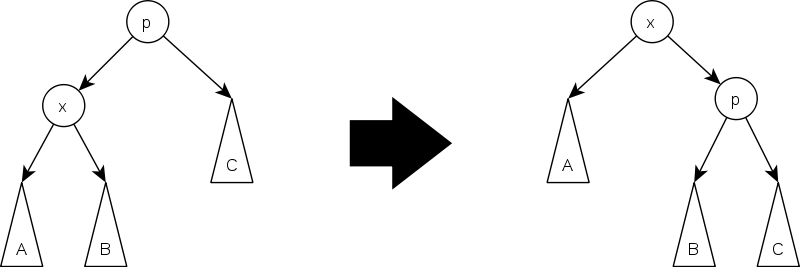
\includegraphics[width=0.75\textwidth]{Zig.png}
  \caption{\textbf{Zig.} Rotate self (at top of tree).}
\end{figure}

\begin{figure}
  \center
  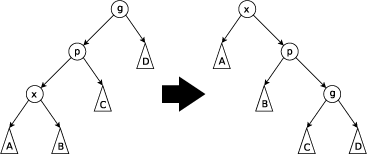
\includegraphics[width=0.75\textwidth]{Zigzig.png}
  \caption{\textbf{Zig-zig.} Rotate parent, then rotate self.}
\end{figure}

\begin{figure}
  \center
  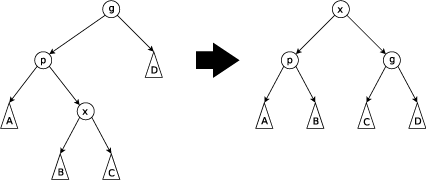
\includegraphics[width=0.75\textwidth]{Zigzag.png}
  \caption{\textbf{Zig-zag.} Rotate self twice.}
\end{figure}

\end{document}
